
\chapter{Case Study: Data Structure Selection}
\label{data_struct_sel}

At this point you have learned about Raku's core data structures,
and you have seen some of the algorithms that use them.

This chapter presents a case study with exercises that let
you think about choosing data structures and practice using them.

But first, I would like to briefly introduce two conditional 
structures that have been left aside so far and provide 
a couple of new possibilities about subroutine signatures. 
\index{signature}

\section{The Ternary Conditional Operator}
\label{ternary operator}
\index{ternary conditional operator}

Consider the following code that tests the value of a positive 
integer:

\begin{verbatim}
my $result;
if $num < 10 {
    $result = "One digit";
} else {
    $result = "More than one digit";
}
say $result;
\end{verbatim}

This is quite simple, but a bit long. This can be rewritten 
in just one line of code:

\begin{verbatim}
say $num < 10 ?? "One digit" !! "More than one digit";
\end{verbatim}

The operator is in two parts: the {\tt ??} and the {\tt !!}, which 
separate three expressions (hence the name ``ternary operator''): 
\index{ternary operator}
\index{operator!ternary}
\begin{itemize}
\item The condition to be evaluated (is \verb'$num' less than 10?);
\item The expression defining the value if the condition is true;
\item The expression defining the value if the condition is false.
\end{itemize}

This statement checks if \verb'$num' is less than 10 and, if 
true, prints ``"One digit;'' if the 
condition is false, it prints ``More than one digit.''

This operator does not provide any new functionality; it just 
offers a more concise syntax.

It is possible to nest several ternary operators to examine 
successively multiple choices:
\index{ternary conditional operator, nesting}

\begin{verbatim}
say $value < 10    ?? "One digit"     !! 
    $value < 100   ?? "Two digits"    !!
    $value < 1000  ?? "Three digits"  !!
                      "More than three digits";
\end{verbatim}

This construct is a form of what is sometimes called a 
\emph{switch statement}, because the C language and 
many languages derived from it use the {\tt switch} keyword 
to describe such a multiple choice conditional.
\index{switch statement}

This is much more concise and often more convenient than nested 
{\tt if ... then ... else} conditionals, but the next section 
provides a more powerful {\tt switch} type of statement.

\section{The {\tt given ... when} ``Switch'' Statement}
\label{given_when}
\index{given statement}
\index{when statement}
\index{switch statement}

Raku has a ``switch'' statement, written with the 
{\tt given} and {\tt when} keywords. The 
{\tt given} keyword introduces the variable or expression 
that will be tested, and each of the {\tt when} 
statements specify a condition followed by a block that 
will execute if the condition is true. By default, the 
process stops at the first condition that is satisfied.

The example just above can be rewritten as follows:

\begin{verbatim}
given $value {
    when 0..9      { say "One digit" }
    when $_ < 99   { say "Two digits" }
    when /^\d**3$/ { say "Three digits" }
    default        { say "More than three digits" }
}
\end{verbatim}

The \verb'given $value' statement ``topicalizes'' the argument, 
i.e., assigns the content of  \verb'$value' to the \verb'$_' 
topical variable (or, more precisely, aliases it to \verb'$_'). 
The argument to {\tt given} is a simple variable in the 
example above, but it can be a complex expression whose 
evaluation is stored (and cached) into \verb'$_'. 
Each of the {\tt when} conditions is checked against \verb'$_'. 
I have written these conditions in three different syntactical 
forms to illustrate some of the various possibilities:
\index{topical variable}
\index{alias}
\begin{itemize}
\item The first one checks \verb'$_' (implicitly) against 
the \verb'0..9' range.
\index{range operator}
\item The second one compares explicitly \verb'$_' to 99.
\item The third one uses a regex to check whether \verb'$_' has 
three digits.
\index{regex}
\item The \verb'default' statement runs only if the other 
conditions have failed.
\index{default statement}
\end{itemize}

Only one message will be printed, because the 
matching process stops as soon as one condition has been 
satisfied, and the \verb'default' clause will run if 
no other condition has been met.

If there is no specific operator in the {\tt when} clause, 
then it will smart match the expression in the {\tt when} 
clause against \verb'$_':
\index{smart match}

\begin{verbatim}
when $foo { ... }
# equivalent to: when $foo ~~ $_ { ... }
\end{verbatim}

Note that the {\tt given} keyword is not doing much more than 
topicalizing its argument for the rest of the block. 
The {\tt when} clauses are doing the bulk of the real work. In fact, 
you could even use the {\tt when} clauses without a {\tt given}, 
provided you assign the right value to \verb'$_', which, as you 
hopefully remember, can be done with a {\tt for} block:
\index{for block}

\begin{verbatim}
my $val = 7;
for $val { 
    when 0..6 { say "less than"}
    when 7 {say "Exact";} 
    when 8..* {say "greater than";}
}
\end{verbatim}

\index{proceed clause}
It is possible to add a {\tt proceed} clause at the end of 
any of the conditional code blocks to prevent the process 
from stopping after that code block has succeeded. For example, 
you might write this:

\begin{verbatim}
given $value {
    when 0..9      { say "One digit"}
    when 10..99    { say "Two digits"; proceed}
    when 42        { say "The response to the ultimate question"}
    when /^\d**3$/ { say "Three digits" }
    default        { say "More than three digits" }
}
\end{verbatim}

Here, if \verb'$value' is 42, two messages will be displayed,  
``Two digits'' and ``The response to the ultimate question,'' 
because the {\tt proceed} clause in the second code block 
prevents the process from stopping on the first successful match.

Good, it seems, but there is a problem. The {\tt proceed} clause 
should be used with some care, as it can easily lead 
to unexpected results. In fact, \emph{the code above 
is actually wrong}: if \verb'$value' has two digits but is 
not 42 (if it is, say, 43), the default block will also run, 
because the only other successful match had this {\tt proceed} 
clause, and will say that there are ``More than three digits'' 
although this is obviously false. 

\label{proceed_ex}
As an exercise, test the above code with various values and 
try to find a way to fix the bug with the {\tt proceed} 
clause.

Solution: \ref{sol_proceed_ex}

\section{Multiple Conditionals with Junctions}
\label{junction}
\index{junction}

Sometimes, you need to test several possible conditions 
and would write something like this:

\begin{verbatim}
if $value == 3 or $value == 5 or $value == 7 { #...
\end{verbatim}

This is quite verbose, and I don't like to have to 
repeat the \verb'$value ==' part several times. I 
would prefer to be able to write something like: 
``If value is 3 or 5 or 7.'' That syntax doesn't work, 
but junctions enable you to do almost that:

\begin{verbatim}
if $value == 3|5|7 {
	say "$value is either 3, or 5, or 7"
}
\end{verbatim}

The \verb'3|5|7' part is a junction.

Junctions are superpositions of unordered values. 
Operations on junctions are executed for each item 
of the junction separately (and maybe even in parallel), 
and the results are assembled in a junction of the same 
type.

The junction types differ when evaluated in boolean context. 
The types and associated junction constructors are 
\verb'any', \verb'all', \verb'one' and \verb'none'.
\index{any junction}
\index{all junction}
\index{none junction}
\index{one junction}

\begin{verbatim}
Type  Constructor  Infix    True if ...
                  Operator
any   any            |      at least one value evaluates to True
all   all            &      no value evaluates to False
one   one            ^      exactly one value evaluates to True
none  none                  no value evaluates to True

\end{verbatim}

\index{junction types}

For example, \verb'3|5|7' is the same as \verb'any(3, 5, 7)'.

This is another example of an \verb'any' junction:

\begin{verbatim}
my Junction $weekday = any <Monday Tuesday Wednesday 
                            Thursday Friday>
if $day eq $weekday {
    say "This is a weekday";
}
\end{verbatim}

In this example the \verb'eq' operator is called with each 
pair \verb'$day', 'Monday', \verb'$day', 'Tuesday', etc. 
and the result is put into an any-junction again. As 
soon as the result is determined (in this case, as soon 
as one comparison returns True), it can abort the 
execution of the other comparisons.

This works not only for operators, but also for routines:

\begin{verbatim}
if 2 == sqrt(4 | 9 | 16) {
    say "YaY";
}
\end{verbatim}

Junctions can be very handy to perform fairly common tasks. 
Imagine you have an array of numbers, and you want to 
check that all of them are non-negative. In most 
programming languages, you would write a loop to 
iterate over the array and check each item in turn. 
In Raku, this is very simple:

\begin{verbatim}
my @values = get-values();
if all(@values) >= 0 { ... }
\end{verbatim}

Or, if you want to avoid a division by zero exception:

\begin{verbatim}
my @values = get-values();
perform-division(@values) if none(@values) == 0;
\end{verbatim}
\index{junction}

\section{Subroutine Named and Optional Parameters}

The subroutines that we have seen so far used \emph{positional} 
parameters, i.e., parameters whose binding with the subroutine 
call arguments rely on their order within the list of 
arguments and in the signature. This is usually fine when 
the number of arguments passed to the subroutine is small 
(say, three or less). 
\index{positional parameter}
\index{parameter!positional}
\index{signature}

When the subroutine signature becomes longer, using positional 
arguments might become cumbersome and error-prone. 

\subsection{Named Parameters}
\index{named parameter}
\index{parameter!named}

Named arguments may be supplied in any order: the name of 
the parameter is bound to the argument having the same 
name. For example:

\begin{verbatim}
sub divide (:$dividend, :$divisor where $divisor != 0) {
     return $dividend/$divisor;
}
say divide(dividend => 2048, divisor => 128);      # -> 16
# or:
say divide(divisor => 128, dividend => 2048);      # -> 16
\end{verbatim}

The arguments are supplied at the subroutine call as a list of 
pairs using the pair-constructor syntax. In the signature, 
the parameters are retrieved with the 
so-called colon-pair syntax: the \verb'$dividend' parameter is 
bound to the value of the pair whose key is ``dividend'' (2048), 
and \verb'$divisor' is similarly bound to 128, irrespective of 
the order of the arguments in the subroutine call.
\index{colon-pair syntax}
\index{pair constructor}

These named parameters are especially useful when the number of 
arguments is large. For example, we haven't covered 
object-oriented programming yet (see Chapter~\ref{objects}), 
but this is how we could create an object of the 
(user-defined) Rectangle class:

\begin{verbatim}
my $rect = Rectangle.new( 
    origin_x  => 100, 
    origin_y  => 200, 
    width     => 23,
    length    => 42,
    color     => 'black'
);
\end{verbatim}

Clearly, using five positional parameters would be unpractical. 

\subsection{Optional Parameters}
\index{optional parameter}
\index{parameter!optional}
\index{variadic subroutine}
\index{signature}

Sometimes, the actual number of arguments is not known 
in advance: for example, a subroutine may be called with 
a variable number of arguments. Such a subroutine is said 
to be \emph{variadic}. You can define a parameter to be 
optional by postfixing it with a question mark in the 
subroutine signature:

\begin{verbatim}
sub my-sub($x, $y?) {  # simple optional parameter
    if $y.defined {
        say "The second parameter has been supplied and defined";
    } else {
        say "The second parameter has not been supplied";
    }
    # ...
}
\end{verbatim}

\index{positional parameter}
\index{parameter!positional}
When using positional parameters, the optional parameters 
always have to be the last ones in the list (after the 
mandatory ones).

A parameter can also be made optional by supplying a 
{\bf default value}:
\index{default value}
\index{default parameter}
\index{parameter!default value}

\begin{verbatim}
sub my-log($number, $base = e) {    # e is a predefined constant
                                    # $base is an optional parameter
    return log($number) / log($base);
}
say my-log(4);       # Natural log (base e)    -> 1.38629436111989
say my-log(32, 2);   # Log base 2              -> 5
say my-log(100, 10); # Common log (base 10)    -> 2
\end{verbatim}

Here, if the second argument is not supplied, the default 
value (\emph{e}) is used instead. Conversely, if there 
is a second argument, it {\bf overrides} the default value.

\index{slurpy parameters}
\index{parameter!slurpy}
\label{slurpy_parameters}
Sometimes, having optional or default parameters is not good 
enough. For example, the subroutine may have to process a list 
containing any number of values. For situations like this, 
you can use a \emph{slurpy parameter}, i.e., a kind of array 
placed at the end of the parameter list that will slurp up 
all the remaining arguments. This kind of slurpy parameter 
uses the ``\verb"*@"'' twigil. In the following example, 
the subroutine takes one mandatory parameter (the first 
number of the list) and a list of additional arguments 
that will be stored in the \verb'@rest' array:
\index{twigil}

\begin{verbatim}
sub my-sum($first-num, *@rest) {
    say @rest;                      # -> [3 4 5 12 17]
    return $first-num + [+] @rest;
}
say my-sum 1, 3, 4, 5, 12, 17;      # -> 42 
\end{verbatim}

Some further examples of slurpy parameters have been 
provided in Section~\ref{sol_exercise_queue}.

\section{Word Frequency Analysis}
\label{analysis}

Now, let's get to the case study.

As usual, you should at least attempt the exercises
before you read the suggested solutions, which are 
provided in the following sections of this chapter.

\begin{exercise}

Write a program that reads a file, breaks each line into
words, strips whitespace and punctuation from the words, and
converts them to lowercase.

\end{exercise}


\begin{exercise}
\index{Project Gutenberg}

Go to Project Gutenberg (\url{http://gutenberg.org}) and download 
your favorite out-of-copyright book in plain text format.
\index{plain text}
\index{text!plain}

Modify your program from the previous exercise to read the book
you downloaded, skip over the header information at the beginning
of the file, and process the rest of the words as before.

Then modify the program to count the total number of words in
the book, and the number of times each word is used.
\index{word frequency}
\index{frequency!word}

Print the number of different words used in the book.  Compare
different books by different authors, written in different eras.
Which author uses the most extensive vocabulary?
\end{exercise}


\begin{exercise}

Modify the program from the previous exercise to print the
20 most frequently used words in a given book.

\end{exercise}


\begin{exercise}

Modify the previous program to read a word list (see
Section~\ref{wordlist}) and then print all the words in the book that
are not in the word list.  How many of them are typos?  How many of
them are common words that {\em should} be in the word list, and how
many of them are really obscure?

\end{exercise}


\section{Random Numbers}
\index{random number}
\index{number, random}
\index{deterministic}
\index{pseudorandom}

Given the same inputs, most computer programs generate the same
outputs every time, so they are said to be {\bf deterministic}.
Determinism is usually a good thing, since we expect the same
calculation to yield the same result.  For some applications, though,
we want the computer to be unpredictable.  Games are an obvious
example, but there are more.

Making a program truly nondeterministic turns out to be difficult,
but there are ways to make it at least seem nondeterministic.  One of
them is to use algorithms that generate {\bf pseudorandom} numbers.
Pseudorandom numbers are not truly random because they are generated
by a deterministic computation, but just by looking at the numbers it
is all but impossible to distinguish them from random.

Raku provides functions such as {\tt rand} that generate
pseudorandom numbers (which we will simply call ``random'' 
numbers from here on).
\index{rand function}
\index{function!rand}

The function {\tt rand} returns a random number (of {\tt Num} 
type) between 0.0 and 1.0 (including 0.0 but not 1.0).  Each time you
call {\tt rand}, you get the next number in a long series.  To see a
sample, run this loop in the REPL:

\begin{verbatim}
say rand for 1..5;
\end{verbatim}

Used as a method, {\tt rand} returns a random number between 
0.0 and the value of the invocant. For example, {\tt 10.rand} 
returns a random number between 0 and 10 (10 not included). You
might try it as a one-liner:
\index{one-liner mode}

\begin{verbatim}
$ raku -e 'say 10.rand for 1..5'
8.23987158729588
9.83276889381497
2.52313276833335
3.44713459548771
1.82329894347025
\end{verbatim}
 
You should hopefully get a different output than I did. If 
you want to run such a one-liner under Windows, remember 
that you'll need to replace single quotes with double quotes.

To obtain random integers between 1 and 10, you may use 
the {\tt Int} and {\tt rand} methods:
\index{Int function or method}

\begin{verbatim}
$ raku -e 'say 10.rand.Int + 1 for 1..5'
5
10
1
6
3
\end{verbatim}

The {\tt pick} function or method takes a number \verb'$count'  and a list as arguments and returns \verb'$count' items chosen at 
random and without repetition. For example:
\index{pick function or method}

\begin{verbatim}
> say <1 3 4 5 7 9 10 12 14 42>.pick(5);
(5 42 3 4 7)
> say pick 5, <1 3 4 5 7 9 10 12 14 42>;
(42 12 5 1 9)
\end{verbatim}

If \verb'$count' if greater than or equal to the number of 
items of the list, then all elements from the list are returned 
in a random sequence.

To obtain random unique integers in a range, you might use 
{\tt pick} on a range:

\begin{verbatim}
> say pick 5, 1..20;
(5 3 6 18 7)
> say (1..20).pick(5);
(20 4 18 2 7)
\end{verbatim}

If you don't specify the number of random numbers, you'll get one 
random pick:

\begin{verbatim}
> say (1..20).pick;
19
\end{verbatim}
%


\begin{exercise}
\index{histogram!random choice}

Write a function named \verb"choose_from_hist" that takes
a histogram as defined in Section~\ref{histogram} and returns a 
random value from the histogram, chosen with probability
in proportion to frequency.  For example, for the three 
items: \verb"('a', 'a', 'b')", your function should 
return \verb"'a'" with probability $2/3$ and \verb"'b'" 
with probability $1/3$.
\end{exercise}


\section{Word Histogram}

You should attempt the previous exercises before you go on.

For the purpose of presenting the solutions to the above 
exercises, I've used the plain text of {\em Emma} (1816), the 
novel by Jane Austen, downloaded from the Gutenberg project 
(\url{http://www.gutenberg.org/files/158/158-0.txt}) and 
saved in a file called \emph{emma.txt} \footnote{The Gutenberg 
project slightly modified the format of this file after this 
chapter was written. To avoid any problem associated with this 
change (and any other future changes), you can download the 
original file from my Github repository: 
\url{https://github.com/LaurentRosenfeld/think_raku/blob/master/Supplementary/emma.txt}.} Use the same 
text if you want to compare your solutions and results 
with mine.
\index{Austin, Jane}
\index{Emma}
\index{Project Gutenberg}

Here is a program that reads the \emph{emma.txt} file and 
builds a histogram of the words in the file:
\index{histogram!word frequencies}

\begin{verbatim}
my %histogram;
my $skip = True; # flag to skip the header

sub process-line(Str $line is copy) {
    if defined index $line, "*END*THE SMALL PRINT!" {
        $skip = False ;
        return;
    }
    return if $skip;
    $line ~~ s:g/<[-']>/ /; # Replacing dashes and apostrophes with spaces
    $line ~~ s:g/<[;:,!?.()"_`]>//; # removing punctuation symbols
    $line = $line.lc;               # setting string to lower case
    for $line.words -> $word {
        %histogram{$word}++;
    }
	$skip = True if $line ~~ /^finis$/;
}
process-line $_ for "emma.txt".IO.lines; 
\end{verbatim}
\index{case!lower}
%

The program reads each line of the \emph{emma.txt} file and, for 
each line, calls \verb"process-line". 

\index{accumulator!histogram}
The \verb"process-line" subroutine skips the header lines 
(i.e., all the lines until a line containing the string
``*END*THE SMALL PRINT!'' 
is met \footnote{This line is no longer present in the new version of 
the Emma file currently on the Gutenberg project site. So this will 
work only with my version of this file on my Github repository:  
\url{https://github.com/LaurentRosenfeld/think_raku/blob/master/Supplementary/emma.txt}.}). It replaces dashes and apostrophes with spaces, removes 
various punctuation characters, and sets the line to lower case. 
Finally, it splits the line into individual words that are 
stored and counted with an accumulator in the \verb'%histogram' 
hash.

To know whether the program is doing something like what 
it is supposed to do, we can display a few entries of the 
\verb'%histogram' hash:

\begin{verbatim}
# displaying 20 lines of the histogram
my $count;
for %histogram -> $pair {
    say sprintf "%-24s %d", $pair.key, $pair.value;
    $count++;
    last if $count > 20;
}
\end{verbatim}

This prints out the following output:

\begin{verbatim}
embarrassing             1
hows                     1
appealed                 2
bestow                   2
articulate               1
demands                  2
closely                  1
dull                     9
hearts                   1
column                   1
possesses                1
attributed               1
jumped                   2
forwards                 2
wittier                  2
expert                   2
attractive               2
asserted                 2
oftentimes               1
fancy                    38
finds                    1
\end{verbatim}


To count the total number of words in the file, we can add up
the values in the histogram:

\begin{verbatim}
my $word_count = [+] %histogram.values;
say "There are $word_count words in the book.";
\end{verbatim}
%
The number of different words is just the number of items in
the hash:

\begin{verbatim}
my $distinct-words = %histogram.elems;
say "There are $distinct-words distinct words in the book.";
\end{verbatim}
%
Note that you could reduce the above to one code line by 
interpolating a code block within the output string:
\index{interpolating a code block in a string}

\begin{verbatim}
say "There are {%histogram.elems} distinct words in the book."
\end{verbatim}
%
And the results:

\begin{verbatim}
There are 161991 words in the book.
There are 7110 distinct words in the book.
\end{verbatim}
%


\section{Most Common Words}
\label{most_common_words}

To find the most common words in \verb'emma.txt', we can 
sort the \verb'%histogram' hash according to the values 
(word frequencies) and retrieve the 10~most frequent words 
into an array.
\index{sort}

\begin{verbatim}
my @most_commons = (sort { %histogram{$^b} cmp %histogram{$^a} }, 
                    %histogram.keys)[0..9];
say $_ for map { "$_ \t%histogram{$_} "}, @most_commons;
\end{verbatim}

The {\tt sort} functions receives the keys of the histogram and 
its comparison function compares the values associated with 
those keys. Since we use the key \verb'$^b' before the key 
\verb'$^a', the sort will produce a reverse (descending) sort 
order. The whole {\tt sort} procedure is placed within parentheses, 
so that the subscript range {\tt [0..9]} acts as a slice on 
the list produced by {\tt sort} and retains only the first 10~most 
frequent words. The result is stored into the 
\verb'@most_commons' array. The next code line just reprocesses 
the array to display the words and their respective frequency.
\index{slice}

This displays the following output:

\begin{verbatim}
to      5241
the     5205
and     4897
of      4295
i       3192
a       3130
it      2529
her     2490
was     2400
she     2364
\end{verbatim}
%
If you want to see more interesting words, you might, as a
further exercise, filter the histogram and retain only 
words that have more than, say, four letters.

The \verb'@most_commons ' temporary array is not really needed. 
We could do the whole thing in a single statement:

\begin{verbatim}
say $_ for map { "$_ \t%histogram{$_} "},  
           (sort { %histogram{$^b} cmp %histogram{$^a} }, 
           %histogram.keys)[0..9];
\end{verbatim}

This is an example of data pipeline (or stream) programming. Such a statement 
needs to be read from bottom to top and from right to left. The 
first step is \verb'%histogram.keys', which produces a list 
of the histogram keys; this list is fed into the sort statement 
to produce a list of the keys sorted (in descending order) according 
to their values; once this whole part between parentheses is 
completed, the subscript range \verb'[0..9]' retains the 
10~most frequent words and feeds them into the map statement, 
which produces the list of words and frequencies for the final 
output.

Let me add one word of caution here: sorting the histogram by 
values and picking up the top 10 to get the most frequent 
words is probably the easiest way to solve the problem and the 
shortest code to do it. That's the reason I have used this 
solution here. But it is not the most efficient solution 
from the standpoint of the run time, because it involves the 
cost of sorting a relatively large data set, whereas we are 
using only a small part of the sorted data. There are some 
better algorithms to do that from the standpoint of runtime 
efficiency, but they are more complicated. So, there is a 
tradeoff here between coding efficiency and performance. 
Assuming this is code that we want to run only once, I have 
chosen to favor coding efficiency.

\index{data pipeline programming}


\section{Optional Parameters}
\index{optional parameter}
\index{parameter!optional}

We saw earlier in this chapter that subroutines can 
take optional parameters. We can use this functionality to 
write a subroutine that prints the most common words in the 
\verb'%histogram' hash extracted from \emph{emma.txt}.

\begin{verbatim}
display-most-common(%histogram, 5);

sub display-most-common (%hist, Int $num = 10) {
    say $_ for map { "$_ \t%hist{$_} "}, 
    (sort { %hist{$^b} cmp %hist{$^a} },
    %hist.keys)[0..$num - 1];
}
\end{verbatim}

This will display the five top words of the list above 
(Section~\ref{most_common_words}). If we call it without 
the second parameter:

\begin{verbatim}
display-most-common(%histogram);
\end{verbatim}

we will get the 10~most common words (same list as the one 
shown in Section~\ref{most_common_words} above), because 
the default value for the second parameter is 10.


\section{Hash Subtraction}
\label{hashsub}
\index{hash!subtraction}
\index{subtraction!hash}

Finding the words from \emph{emma.txt} that are not in the word list
{\tt words.txt} is a problem you might recognize as set
subtraction; that is, we want to find all the words from one
set (the words in \emph{emma.txt}) that are not in the other (the
words in \emph{words.txt}).

{\tt subtract} takes hashes \verb'%main' and \verb'%dict' and 
returns a new hash that contains all the keys from \verb'%main' 
that are not in \verb'%dict'.  Since we don't really care about 
the values, we set them all to 1:

\begin{verbatim}
sub subtract (%main, %dict) {
	my %difference;
	for %main.keys -> $word {
		%difference{$word} = 1 unless %dict{$word}:exists;
	}
	return %difference;
}
\end{verbatim}
%
To find the words in \emph{emma.txt} that are not in  \emph{words.txt},
we need to load the word list into a hash and to call 
{\tt subtract}, passing the two hashes as arguments. We also 
add some code to print the first 20~words not found in the 
word list:

\begin{verbatim}
my %word-list = map { $_ => 1 }, "words.txt".IO.lines;
my %unknown-words = subtract(%histogram, %word-list);
say %unknown-words.keys.head(20);
\end{verbatim}
%
\index{head}
Notice that rather than using a subscript slice, I have used 
here the {\tt head} method to print out the first 20~words of 
the list. This is just another way to get the first ``n'' items 
of a list or array. There is also a {\tt tail} method to 
retrieve the last ``n'' items of a list or an array.
\index{head method}
\index{tail method}

Here are some of the results from {\em Emma}:

\begin{verbatim}
(penetrated unsullied bateses outstepped particularity experienced 
italian sunday solicitously blockhead unbleached ult 26th 
christian 7th untouched iii greensward houseroom tete)
\end{verbatim}
%
Some of these words are names and ordinal numbers.  Others 
are rare or no longer in common use.  But a few are common
words that should really be in the list!

Note that I have used a hash (\verb'%unknown-words') here to 
store the words of \emph{emma.txt} not found in the word list. 
Since we are using the data only to print a sample of 20 words, 
we could have used an array as well.

\section{Constructing New Operators}

\label{operator_construction}
\index{hash!subtraction}
\index{creating new operators}
\index{new operators!creating}
\index{overload operators}
\index{operator!overloading}
\index{operator construction}

Learning about hash subtraction is an excellent 
opportunity to introduce a very interesting functionality of 
Raku: the capacity to construct new operators or to 
redefine existing ones.

Since we are subtracting two lists of words, it is tempting to 
use the minus sign to denote this subtraction operation. It  
is very easy to create such an operator in Raku:

\begin{verbatim}
multi sub infix:<-> (%main, %dict) {
	my %difference;
	for %main.keys -> $word {
		%difference{$word} = 1 unless %dict{$word}:exists;
	}
	return %difference;
}
\end{verbatim}

\index{infix}
\index{subroutine signature}
\index{signature}
\index{multi!subroutine}

Compared to the definition of the {\tt subtract} subroutine, the 
only differences are in the header line. We will cover the 
details in a later chapter, but let us briefly explain here.
Most Raku operators are defined as ``multi'' subroutines, 
i.e., subroutines that can be defined several times with 
different signatures and bodies; Raku will know which one to use depending 
on the signature. Here we define the minus operator as a 
multi subroutine whose parameters are two hashes; this will be 
enough for the Raku compiler to know that we don't want 
the regular subtraction between numerical values, but something 
else that applies to two hashes. The minus operator is defined as 
``infix,'' which means that the operator will be placed 
between its two operands.

Calling this new operator is now just as easy as calling 
the regular subtraction operator between numbers; we just need 
to use two hashes as operands:

\begin{verbatim}
my %unknown-words = %histogram - %word-list;
\end{verbatim}

The rest of the program works just as before.

\index{extending the language}
This ease or creating new operators is one of the facilities 
offered by Raku to \emph{extend the language} from within itself. 
We'll come back to that and other ways to extend the language 
in later chapters.

\label{fact_operator}
\index{factorial}
\index{factorial!operator}
As an exercise, write a multi subroutine that creates the new 
postfix ``!'' operator for computing the factorial of an integer:
\index{factorial}

\begin{verbatim}
say 5!;     # -> 120
\end{verbatim}
%
Also try to think about how you would test this new ``!'' operator 
against various input values.
Solution: \ref{sol_fact_operator}


\section{Sets, Bags and Mixes}
\label{sets_and_bags}

\index{set}
\index{type!set}
\index{bag}
\index{type!bag}
\index{mix}
\index{type!mix}
\index{sethash}
\index{type!sethash}
\index{baghash}
\index{type!baghash}
\index{mixhash}
\index{type!mixhash}

Raku has a variety of data structure types called {\tt Set}, 
{\tt Bag} and {\tt Mix} that provide many common set 
operations. They are unordered collections of unique and 
weighed items. They are immutable (but there also exist mutable 
versions of these data structures, {\tt SetHash}, {\tt BagHash} 
and {\tt MixHash}).

You may create and use a set as follows:

\begin{verbatim}
> my $s = set <banana apple orange orange banana pear apple>;
set(banana, orange, apple, pear)
> say $s.perl
set("banana","orange","apple","pear")
> say $s.elems;
4
> say $s{'apple'}
True
> say $s{'strawberry'}
False
\end{verbatim}
%
As you can see, duplicates have been removed. Sets only tell us 
whether or not at least one item of a given name has been seen.

A bag, by contrast, also keeps track of how many of each items 
have been seen:

\begin{verbatim}
> my $b = bag <banana apple orange orange banana pear apple orange>;
bag(banana(2), orange(3), pear, apple(2))
> say $b{'banana'}
2
\end{verbatim} 

Mixes are similar to bags, except that the elements' weights don't 
have to be integers.

The interesting thing about these collections is that they can use 
many set operators commonly used in mathematics, such as the 
\verb'∈' set membership operator (or use \verb'(elem)' instead 
if you don't know how to type \verb'∈' in your 
editor~\footnote{I can't teach you here how to type these characters, 
because each editor will require a different method.}), the \verb'∩' or 
\verb'(&)' set intersection operator, or the \verb'⊂' or 
\verb'(<)' subset operator:

\begin{verbatim}
> say "Found it!" if 'apple' ∈ $s;
Found it!
> say "Is subset!" if <orange banana> ⊂ $s;
Is subset!
> say <orange banana pineapple> ∩ $s;
set(banana, orange)
\end{verbatim}

Notice that we haven't used the {\tt set} keyword to define the 
\verb'<orange banana>' list in the second example above. This list 
has been coerced to a {\tt Set} to check whether it was a subset 
of the \verb'$s' set. This is one of the great things about these 
collections: most of these set operators can be used with lists, 
arrays, and hashes.
\index{coercion}

\index{set!membership operator}
\index{operator!set membership}
We can rewrite the hash subtraction program using a set for 
the word list and the  \verb'∈' (or \verb'(elem)') 
set membership operator:

\begin{verbatim}
my %histogram;
my $skip = True; # flag to skip the header
sub process-line(Str $line is copy) {
    # (same as above)
}

process-line $_ for "emma.txt".IO.lines; 
my $word-list = set "words.txt".IO.lines;
my %unknown-words = subtract(%histogram, $word-list);
say %unknown-words.keys.head(20);

sub subtract (%main, $dict) {
	my %difference;
	for %main.keys -> $word {
		%difference{$word} = 1 unless $word ∈ $dict;
	}
	return %difference;
}
\end{verbatim}

The code line in the {\tt for} loop could also be written as follows:

\index{set!contain operator}
\index{operator!set contain}
\begin{verbatim}
        %difference{$word} = 1 unless $word (elem) $dict;
#or:    %difference{$word} = 1 if $word ∉ $dict;
#or:    %difference{$word} = 1 if $word !(elem) $dict;
#or even with the (cont) or ∋ contain operator:
        %difference{$word} = 1 unless $dict (cont) $word;
#or:    %difference{$word} = 1 unless $dict ∋ $word;
#or:    %difference{$word} = 1 if $dict ∌ $word;
# etc.
\end{verbatim}

\index{set!difference operator}
\index{operator!set difference}
The \verb'∖' \footnote{~Note that this is unicode character {\tt 2216}, 
not the same as the $\backslash$ backslash} and \verb'(-)' built-in operators 
provide a set difference, so that we needed neither to write a 
{\tt subtract} subroutine nor to construct our own minus operator:

\begin{verbatim}
process-line $_ for "emma.txt".IO.lines; 
my $word-list = set "words.txt".IO.lines;
my $unknown-words = %histogram.keys (-) $word-list;
say $unknown-words.keys.head(20);
\end{verbatim}

There are more than 30~set operators available, covering most of 
the set operators used in mathematics. I've only shown 
some that are the most likely to be useful. Check into the 
official documentation (\url{https://doc.raku.org/language/setbagmix}) 
if you need some others.

\label{diff_with_set}
As an exercise, you may rewrite the {\tt process-line} 
subroutine or replace it to use a set or a bag instead of a hash 
to store the words of \emph{emma.txt} (and possibly adapt the rest of 
the program where needed), in order to find the words of the \emph{emma.txt} 
that are not in the \emph{words.txt}.
Solution: \ref{sol_diff_with_set}


\section{Random Words}
\label{randomwords}
\index{histogram!random choice}

To choose random words from the histogram, the simplest algorithm
is to build a list with multiple copies of each word, according
to the observed frequency, and then choose from the list with the 
\verb'pick' function:
\index{pick function or method}

\begin{verbatim}
my @array = map {| (.key xx .value)}, %histogram;
say pick 30, @array;
\end{verbatim}
%
The expression \verb'map {| (.key xx .value)}' reads each 
pair of the histogram and creates a list with {\tt .value} 
copies of the string in {\tt key}.  The {\tt pick} function 
selects 30 random words from the array.

This algorithm works, but it is not very efficient; each time you
choose one or some random words, it rebuilds the list, which is 
as big as the original book.  An obvious improvement is to build 
the list once and then make multiple selections, but the list 
is still big.

An alternative is:

\begin{enumerate}

\item Use {\tt keys} to get a list of the words in \emph{emma.txt}.
\index{keys function}

\item Build a list that contains the cumulative sum of the word
  frequencies (see Exercise~\ref{cumulative}).  The last item
  in this list is the total number of words in the book, $n$.
  
\item Choose a random number from 1 to $n$.  Use a bisection search
  (see Exercise~\ref{bisection}) to find the index where the random
  number would be inserted in the cumulative sum.
\index{bisection search}

\item Use the index to find the corresponding word in the newly 
created word list.

\end{enumerate}

\begin{exercise}
\label{randhist}
\index{algorithm}

Write a program that uses this algorithm to choose a random 
word from \emph{emma.txt}.  
Solution: \ref{sol_randhist}
\end{exercise}

Note that Raku offers a shortcut to perform the task 
at hand: when used on a bag, {\tt pick} returns a random 
selection of elements, weighted by the values corresponding 
to each key. Ideally, we should have used a bag instead of 
a hash to store our \verb'%histo' histogram, but we did not 
know about bags at the time. We can, however, construct a 
bag from the \verb'%histo' histogram. Consider the following 
example:
\index{bag}

\begin{verbatim}
> my %histo = ( banana => 5, pear => 1, orange => 12);
{banana => 5, orange => 12, pear => 1}
> my $fruit-bag = bag map { $_ xx %histo{$_}}, %histo.keys;
bag(banana(5), orange(12), pear)
> for 1..10 { say $fruit-bag.pick: 5}
(banana orange orange orange orange)
(orange orange banana orange banana)
(orange orange banana orange orange)
(pear orange banana banana orange)
(orange banana orange orange orange)
...
\end{verbatim}

As you can see, the most common item, ``orange,'' has been 
picked more often than the others, and the least common, 
``pear,'' has not been picked up at all before the fourth 
draw. 

As an exercise, you may want to adapt this code to 
choose random words from \emph{emma.txt}.



\section{Markov Analysis}
\label{markov}
\index{Markov analysis}

If you choose words from \emph{emma.txt} at random, you can get a
sense of the vocabulary, but you probably won't get a sentence:

\begin{verbatim}
this the small regard harriet which knightley's it most things
\end{verbatim}
%
A series of random words seldom makes sense because there
is no relationship between successive words.  For example, in
a real sentence you would expect an article like ``the'' to
be followed by an adjective or a noun, and probably not a verb
or adverb.

One way to measure these kinds of relationships is Markov
analysis, which characterizes, for a given sequence of words, 
the probability of the words that might come next.  For example, 
the second chapter of \emph{The Little Prince} (1943), the 
famous novella written by French writer and pioneer aviator 
Antoine de Saint-Exupéry, begins:
\index{The Little Prince (Antoine de Saint-Exupéry)}
\index{Saint-Exupéry, Antoine de}

\begin{quote}
The first night, then, I went to sleep on the sand, a thousand miles from any human habitation. I was more isolated than a shipwrecked sailor on a raft in the middle of the ocean. Thus you can imagine my amazement, at sunrise, when I was awakened by an odd little voice. It said:

 "If you please-- draw me a sheep!"

 "What!"

 "Draw me a sheep!"

 I jumped to my feet, completely thunderstruck. I blinked my eyes hard. I looked carefully all around me. And I saw a most extraordinary small person, who stood there examining me with great seriousness. (...) 

 Now I stared at this sudden apparition with my eyes fairly starting out of my head in astonishment. Remember, I had crashed in the desert a thousand miles from any inhabited region. And yet my little man seemed neither to be straying uncertainly among the sands, nor to be fainting from fatigue or hunger or thirst or fear. Nothing about him gave any suggestion of a child lost in the middle of the desert, a thousand miles from any human habitation. When at last I was able to speak, I said to him:

 "But-- what are you doing here?"

 And in answer he repeated, very slowly, as if he were speaking of a matter of great consequence:

 "If you please-- draw me a sheep..."

 When a mystery is too overpowering, one dare not disobey. Absurd as it might seem to me, a thousand miles from any human habitation and in danger of death, I took out of my pocket a sheet of paper and my fountain-pen. But then I remembered how my studies had been concentrated on geography, history, arithmetic, and grammar, and I told the little chap (a little crossly, too) that I did not know how to draw. He answered me:

 "That doesn't matter. Draw me a sheep..."

 But I had never drawn a sheep. So I drew for him one of the two pictures I had drawn so often. It was that of the boa constrictor from the outside. And I was astounded to hear the little fellow greet it with,

 "No, no, no! I do not want an elephant inside a boa constrictor. A boa constrictor is a very dangerous creature, and an elephant is very cumbersome. Where I live, everything is very small. What I need is a sheep. Draw me a sheep." 
  
\end{quote}
%
In this text,
the word ``draw'' is always followed by the word ``me,'' and 
the phrase ``draw me'' is always followed by ``a sheep.'' And the 
phrase ``a thousand'' is always followed by ``miles,'' but the 
phrase ``a thousand miles'' may be followed by ``from any 
human habitation" or by ``from any inhabited region.''
\index{prefix}
\index{suffix}
\index{mapping}

The result of Markov analysis is a mapping from each prefix
(like ``draw me'' and ``a thousand miles'') to all possible 
suffixes
(like ``a sheep'' and ``from any habitation'' or ``from any inhabited region'').
\index{random text}
\index{text!random}

Given this mapping, you can generate a random text by
starting with any prefix and choosing at random from the
possible suffixes.  Next, you can combine the end of the
prefix and the new suffix to form the next prefix, and repeat.

For example, if you start with the prefix ``draw me,'' then the
next word has to be ``a sheep,'' because the prefix is always 
followed by ``a sheep'' in the text.  If a prefix is ``a thousand 
miles,'' the next suffix might be ``from any habitation'' or ``from any inhabited region.''

In this example the lengths of the prefixes are two or three words, 
but you can do Markov analysis with any prefix length.

\begin{exercise}

Markov analysis:
\label{markov_analysis}
\index{Markov analysis}

\begin{enumerate}

\item Write a program to read a text from a file and perform Markov
analysis.  The result should be a hash that maps from
prefixes to a collection of possible suffixes.  The collection
might be an array, a hash, a set, a bag, etc.; it is up to you 
to make an appropriate choice.  You can test your program with 
prefix length two, but it would be nice to write the program 
in a way that makes it easy to try other lengths.

\item Add a function to the previous program to generate random text
based on the Markov analysis.  Here is an example from {\em Emma}
with prefix length 2:

\begin{quote}
it was a black morning's work for her. the friends from whom 
she could not have come to hartfield any more! dear affectionate 
creature! you banished to abbey mill farm. now i am afraid 
you are a great deal happier if she had no hesitation in 
approving. dear harriet, i give myself joy of so sorrowful an event;
\end{quote}

For this example, the punctuation has been left attached to 
the words. The result is almost syntactically correct, but not 
quite. Semantically, it almost makes sense, but not quite.

What happens if you increase the prefix length?  Does the random
text make more sense?

\item Once your program is working, you might want to try a mash-up:
if you combine text from two or more books, the random
text you generate will blend the vocabulary and phrases from
the sources in interesting ways.
\index{mash-up}

\end{enumerate}

Credit: this case study is based on an example from Kernighan and
Pike, {\em The Practice of Programming}, Addison-Wesley, 1999.

\end{exercise}

You should attempt this exercise before you go on. Then you can
study our solution in Subsection\ref{sol_markov_analysis}.


\section{Data Structures}
\index{data structure}

Using Markov analysis to generate random text is fun, but there is
also a point to this exercise: data structure selection.  In your
solution to the previous exercises, you had to choose:
\index{fun}
\index{data structure selection}

\begin{itemize}

\item How to represent the prefixes.

\item How to represent the collection of possible suffixes.

\item How to represent the mapping from each prefix to
the collection of possible suffixes.

\end{itemize}

The last one is easy: a hash is the obvious choice
for a mapping from keys to corresponding values.
\index{hash}

For the prefixes, the most obvious options are a string or
a list of strings.
\index{string}

For the suffixes,
one option is a list; another is a histogram (hash).
\index{implementation}

How should you choose?  The first step is to think about
the operations you will need to implement for each data structure.
For the prefixes, we need to be able to remove words from
the beginning and add words to the end.  For example, if the current
prefix is ``draw me,'' and the next word is ``a,'' you need
to be able to form the next prefix, ``me a'' in order to find 
the next suffix, ``sheep.''

Your first choice might be an array, since it is easy to add
and remove elements, but we also need to be able to use the
prefixes as keys in a hash, so that sort of rules out arrays.

For the collection of suffixes, the operations we need to
perform include adding a new suffix (or increasing the frequency
of an existing one), and choosing a random suffix.

Adding a new suffix is equally easy for the list implementation
or the hash.  Choosing a random element from a list
is easy; choosing from a hash is harder to do
efficiently (see Exercise~\ref{randhist}).

So far we have been talking mostly about ease of implementation,
but there are other factors to consider in choosing data structures.
One is run time.  Sometimes there is a theoretical reason to expect
one data structure to be faster than other; for example, we mentioned
that a lookup operation is faster for hashes than for arrays,
especially when the number of elements is large.

But often you don't know ahead of time which implementation will
be faster.  One option is to implement both of them and see which
is better.  This approach is called {\bf benchmarking}.  A practical
alternative is to choose the data structure that is
easiest to implement, and then see if it is fast enough for the
intended application.  If so, there is no need to go on.  If not,
there are tools, like {\tt profile} modules, that can identify
the places in a program that take the most time.
\index{benchmarking}
\index{profile module}
\index{module!profile}

The other factor to consider is storage space.  For example, using a
histogram for the collection of suffixes might take less space because
you only have to store each word once, no matter how many times it
appears in the text.  In some cases, saving space can also make your
program run faster, and in the extreme, your program might not run at
all if you run out of memory.  But for many applications, space is a
secondary consideration after run time.

One final thought: in this discussion, we have implied that
we should use one data structure for both analysis and generation.  But
since these are separate phases, it would also be possible to use one
structure for analysis and then convert to another structure for
generation.  This would be a net win if the time saved during
generation exceeded the time spent in conversion.

\section{Building Your Own Data Structures}

Raku has a number of compound types such as arrays and hashes 
that you can combine to construct arrays of arrays, arrays of 
hashes, hashes of arrays, hashes of hashes, arrays of arrays of 
arrays or hashes, and so on, and this is usually sufficient for 
most needs. Sometimes, however, you need something very specific 
that is not built in.

Over the years, computer science has studied and used scores of 
specific data structures such as linked lists, stacks, queues, 
circular lists, trees of numerous kinds, etc. We will briefly 
study a couple of them.

\subsection{Linked Lists}
\label{linked_list}
\index{linked list}

A linked list is a collection of items in which each item holds 
a value (or several values) and a link to the next item of the 
collection. In many programming languages, arrays have a fixed 
size (contrary to Raku in which arrays can usually grow according to 
your needs). In those programming languages, a linked list 
is often used to represent a variable-size collection of items.

We saw in Section~\ref{stacks_queues} how to use arrays 
to build stacks and queues. It was fairly easy. In some 
lower-level programming languages, you would need linked 
lists for that.
\index{stack}
\index{queue}

In Raku, a linked list item may be represented by a pair 
(an object of type \verb'Pair'). The 
following code is a very simple example showing how 
we could implement a stack using a linked list in Raku:
\index{pair}

\begin{verbatim}
sub add-to-stack (Pair $stack-top, $item) {
    my $new-pair = $item => $stack-top;
    return $new-pair;
}

sub take-from-stack (Pair $stack-top) {
    my $new-top = $stack-top.value;
    return $stack-top.key, $new-top;
}

sub create-stack ($item) {
    return $item => Nil;
}

my $stack = create-stack (0);

for 1..5 -> $item {
    $stack = add-to-stack($stack, $item);
}
say "The stack is: ", $stack.perl;

for 1..5 {
    my $value;
    ($value, $stack) = take-from-stack($stack);
    say "$value -- ", $stack;    
}
\end{verbatim}

Once populated, the resulting stack looks like this:
\index{stack}

\begin{verbatim}
5 => 4 => 3 => 2 => 1 => 0 => Nil
\end{verbatim}

This is just given as an example for the construction of a 
linked list. There is usually no need to use anything like 
this in Raku, since it is much easier to implement 
a stack using an array, as seen in Section~\ref{stacks_queues}, 
although the same principle can be used for building more 
advanced data structures.
\index{linked list}

You might still want, as an exercise, to implement a queue 
(see Section~\ref{stacks_queues}) using a linked list. 

\subsection{Trees}
\label{tree}
\index{tree}
\index{node (tree)}
\index{leaf (tree)}
\index{root (tree)}
\index{tree!node}
\index{tree!leaf}
\index{tree!root}
\index{forest}
\index{child node (tree)}
\index{parent node (tree)}

A tree is usually a collection of items in which each 
item (or \emph{node}) holds a value (or possibly 
several values) and two or several 
links to other items of the collection, the children. Think 
of a family tree or a tree of directories on a hard disk 
drive to get the general idea. The ultimate 
nodes that don't have their own children are often called 
the leaves. There is usually only one ultimate grandparent 
node, sometimes called the root (if there is more than one 
ultimate grandparent, then it is not really a tree but 
several trees or a ``forest'').

Dozens of different types of trees have been invented and 
their descriptions have filled entire books about computer 
science algorithms. Some are designed 
to keep the data sorted, others to maintain balance between 
the tree branches, and so on. The data structure is often 
not very complicated, but the algorithms needed to maintain the 
required properties sometimes can be a bit hairy.

For example, a 
typical tree might hold one value and two links, one to 
the left child and one to the right child. You 
might implement such a \emph{binary tree} in a similar way as the 
linked list described above, except that the value 
would no longer be a link to the next element, but an 
array of two elements, the links to the two children. 
Or you could follow more closely the linked list model 
above and have nested pairs. For example, a binary tree 
might look like this:
\index{binary tree}

\begin{verbatim}
my $tree = 1 => (( 2 => 3 ) => (4 => (5 => ((6 => 7) => 8))));
\end{verbatim}

The implementation is left as an exercise to the reader. 

Quite often, though, a tree may be implemented in Raku 
as a simpler data structure such as a nested array or hash. 
The next section examines such an example.

\subsection{Binary Heaps}
\label{heap}
\index{heap}
\index{binary heap}

A binary heap is a binary tree that keeps a partial order: each 
node has a value larger that its parent and less than 
either of its two children; there is no specific order imposed 
between siblings. (You could also do it the other way 
around: you could design heaps in which any node has a value 
less than its parent.)

Because there is no order between siblings, it is not possible 
to find a particular element without potentially searching the 
whole heap. Therefore, a heap is not very good if you need 
random access to specific nodes. But if you're interested 
in always finding the smallest item, then a heap is a 
very efficient data structure.

Heaps are used for solving a number of CS problems, and serve 
as the basis for an efficient and very popular sorting technique 
called heap sort.
\index{heap sort}

For a human, it is useful to represent a heap in a tree-like 
form. But a computer can store a heap as a simple array (not 
even a nested array). For this, the index of an element is 
used to compute the index of its parent or its two children.
The children of an element are the two locations where the 
indices are about double its index; conversely, the parent 
of a node is located at about half its index. If the heap 
starts at index 0, the exact formulas for a node with index 
\verb'$n' are commonly as follows:
\begin{itemize}
\item parent: \verb'int( ($n-1)/2 )'
\item left child: \verb'2*$n + 1'
\item right child: \verb'2*$n + 2'
\end{itemize}
The root node is at index 0. Its children are at positions 
1 and 2. The children of 1 are 3 and 4 and the children of 
2 are 5 and 6. The children of 3 are 7 and 8, and so on.

Thus, if interpreted as a binary heap, the array:
\begin{verbatim}
[0, 1, 2, 3, 4, 5, 6, 7, 8]
\end{verbatim}

is associated with the tree displayed in Figure~\ref{fig.heap}.

\begin{figure}
\centerline
{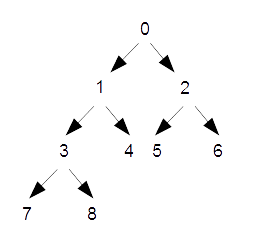
\includegraphics[scale=1]{figs/figure_heap.png}}
\caption{The heap corresponding to an array containing the digits 0 to 8}
\label{fig.heap}
\end{figure}

Here is one way to build a heap (in partial alphabetic order) 
from a list of unordered letters:

\begin{verbatim}
sub build-heap (@array, $index is copy) {
    my $index-val = @array[$index];
    while ($index) {
        my $parent = Int( ($index - 1) / 2);
        my $parent-val = @array[$parent];
        last if $parent-val lt $index-val;
        @array[$index] = $parent-val;
        $index = $parent;
    }
    @array[$index] = $index-val;
}

sub heapify (@array) {
    for @array.keys -> $i {
        build-heap @array, $i;
    }
}

my @input =  <m t f l s j p o b h v k n q g r i a d u e c>; 
heapify @input;
say @input;
\end{verbatim}

Note that the heap is built in place (there is no 
need for a second array). The resulting array is 
displayed as follows:
\begin{verbatim}
[a b g d c k j l f h e m n q p t r o i u s v]
\end{verbatim}

Is this a correct heap? It's difficult to say at first 
glance and checking it manually is somewhat tedious. When 
writing a program for building such a data structure, 
it is often useful to write some subroutines to display 
the content in a way that makes it easier to understand 
the result and check its correctness. The following 
code shows two examples of such possible subroutines:
\begin{verbatim}
sub print-heap (@array) {
    my $start = 0;
    my $end = 0;
    my $last = @array.end;
    my $step = 1;
    loop {
        say @array[$start..$end];
        last if $end == $last;
        $start += $step;
        $step *= 2;
        $end += $step;
        $end = $last if $end > $last;
    } 
}

sub print-heap2 (@array) {
    my $step = 0;
    for @array.keys -> $current {
        my $left_child = @array[2 * $current + 1];
        say "$current\tNode = @array[$current];\tNo child" 
             and next unless defined $left_child;
        my $right_child = @array[2 * $current + 2] // "' '";
        
        say "$current\tNode = @array[$current];\tChildren: " . 
             " $left_child and $right_child";
        $step++;
    }
}
\end{verbatim}

The first one displays the related tree level by level:

\begin{verbatim}
(a)
(b g)
(d c k j)
(l f h e m n q p)
(t r o i u s v)
\end{verbatim}

which makes it easy to draw the tree (see Figure~\ref{fig.heap2}).

\begin{figure}
\centerline
{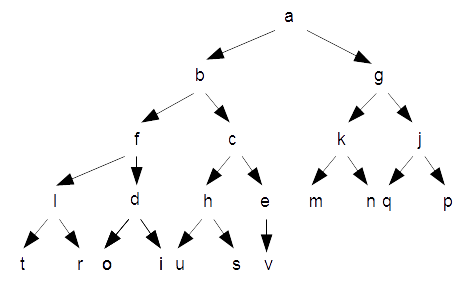
\includegraphics[scale=1]{figs/figure_heap2.png}}
\caption{The heap corresponding to the array of letters}
\label{fig.heap2}
\end{figure}


The second one shows the children for each node and makes it 
possible to easily check that the partial alphabetic order 
constraint is satisfied (i.e., each node is smaller than its 
children):

\begin{verbatim}
0       Node = a;       Children:  b and g
1       Node = b;       Children:  d and c
2       Node = g;       Children:  k and j
3       Node = d;       Children:  l and f
4       Node = c;       Children:  h and e
5       Node = k;       Children:  m and n
6       Node = j;       Children:  q and p
7       Node = l;       Children:  t and r
8       Node = f;       Children:  o and i
9       Node = h;       Children:  u and s
10      Node = e;       Children:  v and ' '
11      Node = m;       No child
12      Node = n;       No child
(...)
21      Node = v;       No child
\end{verbatim}



\section{Debugging}
\index{debugging}

When you are debugging a program, and especially if you are
working on a hard bug, here are some things to try:

\begin{description}

\item[Reading] Examine your code, read it back to yourself, and
check that it says what you meant to say.

\item[Running] Experiment by making changes and running different
versions.  Often if you display the right thing at the right place
in the program, the problem becomes obvious, but sometimes you have to
build scaffolding.

\item[Running under a debugger] A {\bf debugger} is a utility 
program that enables you to run a program step by step, 
so you can follow the execution path and check the content of important 
variables at crucial points in the program execution, to set 
break points, etc. Raku provides a debugger, called 
{\tt raku-debug}, that makes all these things possible. With the 
advent of modern high-level languages, many people balk at 
using a debugger. This is a mistake. A debugger will not help 
solve every kind of problem, but it can be immensely 
useful. See Section~\ref{raku-debugger} for more information
on the Raku debugger.
\index{debugger}

\item[Ruminating] Take some time to think!  What kind of error
is it: syntax, runtime, or semantic?  What information can you get from
the error messages, or from the output of the program?  What kind of
error could cause the problem you're seeing?  What did you change
last, before the problem appeared?

\item[Rubber ducking] If you explain the problem to someone else, you
sometimes find the answer before you finish asking the question.
Often you don't need the other person; you could just talk to a rubber
duck.  That's the origin of the well-known strategy called {\bf
rubber duck debugging}.  I am not making this up; see 
\url{https://en.wikipedia.org/wiki/Rubber_duck_debugging}.
\index{rubber duck debugging}

\item[Retreating] At some point, the best thing to do is back
off, undoing recent changes, until you get back to a program that
works and that you understand.  Then you can start rebuilding.

\end{description}

Beginning programmers sometimes get stuck on one of these activities
and forget the others.  Each activity comes with its own failure
mode.
\index{typographical error}

For example, reading your code might help if the problem is a
typographical error, but not if the problem is a conceptual
misunderstanding.  If you don't understand what your program does, you
can read it 100 times and never see the error, because the error is in
your head.
\index{experimental debugging}

Running experiments can help, especially if you run small, simple
tests.  But if you run experiments without thinking or reading your
code, you might fall into a pattern we call ``random walk programming,'' 
which is the process of making random changes until the program
does the right thing.  Needless to say, random walk programming
can take a very long time.
\index{random walk programming}
\index{development plan!random walk programming}

You have to take time to think.  Debugging is like an
experimental science.  You should have at least one hypothesis about
what the problem is.  If there are two or more possibilities, try to
think of a test that would eliminate one of them.

But even the best debugging techniques will fail if there are too many
errors, or if the code you are trying to fix is too big and
complicated.  Sometimes the best option is to retreat, simplifying the
program until you get to something that works and that you
understand.

Beginning programmers are often reluctant to retreat because
they can't stand to delete a line of code (even if it's wrong).
If it makes you feel better, copy your program into another file
before you start stripping it down.  Then you can copy the pieces
back one at a time.

Finding a hard bug requires reading, running (with or without 
a debugger), ruminating, and sometimes retreating.  If you get 
stuck on one of these activities, try the others.


\section{Glossary}

\begin{description}

\item[Deterministic] Pertaining to a program that does the same
thing each time it runs, given the same inputs.
\index{deterministic}

\item[Pseudorandom] Pertaining to a sequence of numbers that appears
to be random, but is generated by a deterministic program.
\index{pseudorandom}

\item[Default value] The value given to an optional parameter if no
argument is provided.
\index{default value}

\item[Override] To replace a default value with an argument.
\index{override}

\item[Benchmarking] The process of choosing between various data 
structures and algorithms by implementing alternatives and testing 
them (especially their run durations) on a sample of the possible inputs.  
\index{benchmarking}

\item[Debugger] A program that lets you run your code line by 
line and check its state at any step during its execution.
\index{debugger}

\item[Rubber duck debugging] Debugging by explaining your problem
to an inanimate object such as a rubber duck.  Articulating the
problem can help you solve it, even if the rubber duck 
doesn't know Raku. 
\index{rubber duck debugging}
\index{debugging!rubber duck}

\end{description}



\section{Exercises: Huffman Coding}
\label{huffman_exercise}

Huffman coding is a technique used for data compression, i.e., 
to reduce the size of a piece of data (such as, for example, 
compressing a file).

\subsection{Variable-Length Codes}
\index{variable-length code}

If you are familiar with Morse code, you know that it is a 
system for encoding the letters of the alphabet as a series 
of dots and dashes. For example, the famous signal {\tt ...---...} 
represents the letters SOS, which comprise an 
internationally recognized call for help. The table 
in Figure~\ref{fig.morse} shows the rest of the codes.
\index{Morse code}

\begin{figure}
\centerline
{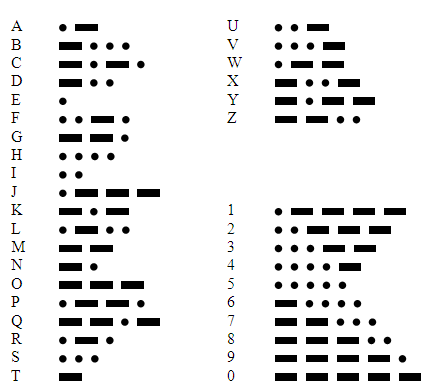
\includegraphics[scale=0.6]{figs/International_Morse_Code.PNG}}
\caption{International Morse code (public domain)}
\label{fig.morse}
\end{figure}

Morse code (invented between 1836 and 1844) was one of the 
very first attempts at digital encoding of the alphabet of a 
plain text. The only known earlier attempt is the braille 
alphabet (1824-1837).
\index{Morse, Samuel}
\index{braille alphabet}

Notice that some codes are longer than others. By design, the 
most common letters have the shortest codes. Since there are a 
limited number of short codes, that means that less common letters 
and symbols have longer codes. A typical message will have more 
short codes than long ones, which minimizes the average 
transmission time per letter.

Codes like this are called variable-length codes. In this exercise, 
we will look at an algorithm for generating a variable-length code 
called a Huffman code. It is an interesting algorithm in its own 
right, but it also makes a useful exercise because its implementation 
uses a variety of data structures.
\index{Huffman!code}

Here is an outline of what we will do until the end of this 
chapter:

\begin{enumerate}

\item First, we will use a sample of English text to generate 
a table of characters and their frequencies.

\item Then we will use this frequency table to generate a code 
table.

\item Finally, we will encode a message with this code table 
and then decode it.

\end{enumerate}

\subsection{The Frequency Table}
\index{frequency!table}

Since the goal is to give short codes to common letters, we 
have to know how often each letter occurs. In Edgar Allan Poe’s 
short story ``The Gold Bug,'' one of the characters, William~Legrand, 
uses letter frequencies to crack a cypher. He explains:
\index{Poe, Edgar Allan}
\index{The Gold-Bug (Edgar Allan Poe)}
\index{cypher}

\begin{quote}
``Now, in English, the letter which most frequently occurs 
is e. Afterwards, the succession runs thus: a o i d h n r s 
t u y c f g l m w b k p q x z. E however predominates so 
remarkably that an individual sentence of any length is 
rarely seen, in which it is not the prevailing character.''
\end{quote}

So our first mission is to see whether Poe got it right. 
To check, let's use as a sample the text of ``The Gold Bug'' 
itself, which can be downloaded from Project Gutenberg 
(\url{http://www.gutenberg.org/files/2147/2147-0.txt}) and 
a variety of other websites. 
\index{Project Gutenberg}

\begin{exercise}
\label{letter_frequency}
Write a program that counts the number of times each letter 
appears in a sample text. Download the text of ``The Gold Bug'' 
and analyze the frequency of the letters.

Solution: see Section~\ref{sol_letter_frequency}
\end{exercise}

\subsection{Building the Huffman Code}
\index{Huffman!code}

For our purposes, Morse code has one defect: it does not 
use just two symbols as you might think, but actually three: 
in addition to the dots and dashes, it it also implicitly 
using the space between two symbols, as well as a longer space 
between two letters.
\index{Morse code}

The reason why some space is needed is quite simple. Refer to the Morse 
code table above and suppose you receive three dots (\verb'...'). 
This could be interpreted as the letter ``e'' three times , or as 
``ie'' or ``ei,'' or as ``s'', or as the beginning of ``h,'' ``v,'' 
``3,'' ``4,'' or ``5''. Added spaces make it possible to disambiguate 
between those various possibilities. But they also make code 
transmission much slower.

In 1951, David A. Huffman invented a code-building technique avoiding 
this problem: provided that you know where a given letter starts, 
it is totally unambiguous. For example, we will meet later a Huffman 
code for a small subset of the alphabet that looks like this:
\index{Huffman, David A.}
\index{Huffman!code}

\begin{verbatim}
a => ..
e => .-
s => -.-
n => -..
t => --.
d => ---.
r => ----
\end{verbatim}

If you start reading a sequence of dots and dashes representing a 
valid text composed with these seven letters, you can always decode 
it without any ambiguity. If the first symbol is a dot, then the letter 
is either an ``a'' or a ``e'' depending on the next symbol. If the 
first symbol is a dash and the next one a dot, then the letter must 
be either a ``s'' or an ``n'' depending on the third symbol. If the 
two first symbols are dashes, you can similarly determine that the 
current letter is a ``t'' (if the third symbol is a dot), or a ``d'' 
or a ``r,'' which you can find out by looking at the fourth symbol. 
In brief, you don't need spaces between the symbols, it is always 
possible to unambiguously decode a letter.

How can we build such a Huffman code? Let's do it by hand with a 
very simple alphabet: the four letters of the nucleo-bases of DNA: A, 
C, T, and G. Suppose we want to encode the following input string:
\index{DNA (deoxyribonucleic acid)}
\index{alphabet}

\begin{verbatim}
CCTATCCTCGACTCCAGTCCA
\end{verbatim}

This gives the following frequency table:
\index{frequency!table}

\begin{verbatim}
C :     10      47.62
T :     5       23.81
A :     4       19.05
G :     2        9.52
\end{verbatim}

To build the Huffman code, we start with the two less frequent 
letters and merge them into one new temporary symbol, \verb"[GA]", 
which we pretend is a new composite letter with a 
frequency of 6. At this point, we decide that, between two letters, 
the less frequent one will have an appended dot and the other 
an appended dash (this is an arbitrary choice, it could be done 
the other way around). So we say that the symbol for the least 
common of the two letters (``G'') will be \verb'[GA].' and the 
symbol for ``A'' will be \verb'[GA]-'. 

We are now left with three letters, C, T, and [GA]. We merge the 
two least frequent letters, ``T'' and ``[GA],'' and can now tell 
that the symbol for ``T'' will be \verb'[TGA].' and the symbol for 
\verb'[GA]' will be \verb'[TGA]-'. There are only two letters left, 
``C'' and ``TGA``, with ``C'' the least frequent one; so ``C'' will 
be a dot and ``TGA`` a dash. 

We can now unroll our dummy letters: ``T'' is \verb'[TGA].', so, 
replacing \verb'[TGA]' with its symbol, i.e., a dash, the 
final code for ``T'' will be \verb'-.'; similarly, \verb'[GA].' 
now translates into \verb'--'. By the same substitution process, 
we can now determine that ``A'' is \verb'---' and ``G'' 
\verb'--.'. So our final Huffman code table is:
\index{Huffman!table}

\begin{verbatim}
C => .
T => -.
G => --.
A => ---
\end{verbatim}

Notice that, by construction, the most frequent letter (C) 
has the shortest code and the least common letters (G and A) 
the longest codes.

Manually encoding the \verb'CCTATCCTCGACTCCAGTCCA' input string 
with this code yields the following pseudo-Morse code:
\index{pseudo-Morse}

\begin{verbatim}
..-.----...-..--.---.-...-----.-...---
\end{verbatim}

Note that our Huffman code is not ambiguous: the first dot can 
only be a ``C,'' and the second one also. The next symbol is a 
dash, which can be the beginning of the three other letters, but 
only ``T'' can have a dot afterwards. The next sequence of 
symbols is four dashes; this can only be the three dashes of a 
``A'', with the last dash being the beginning of the next letter; 
and \verb'-.' can only be a ``T,'' and so on.
\index{Huffman!code}

In a real-life Huffman encoding for text file compression, 
we would not use dots and dashes, but 0 and 1 bits; however,  
dots and dashes are just another nice way of representing 
those binary values. So, let's just pretend that dots and dashes 
are really 0 and 1 binary numbers.
\index{binary number}
\index{bit}

\index{data compression}
Did we really achieve data compression? Our pseudo-Morse string has 
38~binary symbols. The original input string had 21 characters 
or bytes, that is 168 bits. The data has been compressed by a 
factor of about 4.4. 
\index{byte}

Is Huffman coding better than a fixed-length code? A string 
representation where each letter would be represented by two 
bits (two bits can represent four letters) would require 
42~symbols. So, yes, we did obtain a better data compression 
than a fixed-length encoding (by about 10\%). This may seem 
to be a small achievement, but this is actually quite good with 
such a small alphabet. With real text data, Huffman coding can 
achieve significant data compression.


\begin{exercise}
\label{huffman_code_2}
\begin{enumerate}
\item Write a program that performs Huffman encoding of a simple string 
of characters. You may start with the DNA example above. Don't 
worry, though, if you don't get the same Huffman table as the one 
above: there can be more than one Huffman code for a given input 
string; but check that you obtain an unambiguous code. 
\index{Huffman!code}
\item Try it with strings having a larger alphabet (you'll probably 
want to start with a relatively small alphabet, because it can 
otherwise be tedious to check the result by hand).
\item Write a subroutine to encode an input string into 
pseudo-Morse using the generated Huffman table.
\index{pseudo-Morse}
\index{alphabet}
\item Write a subroutine to decode the pseudo-Morse output 
you've just generated for the previous question.
\end{enumerate}
%
Solution: see Section~\ref{sol_huffman_code_2}.
\index{Huffman!code}
\end{exercise}

